%%%%%%%%%%%%%%%%%%%%%%%%%%%%%%%%%%%%%%%%%%%%%%%%%%%%%%%%%%%%%%%%%%%%%%%%%%%%%%%%
%2345678901234567890123456789012345678901234567890123456789012345678901234567890
%        1         2         3         4         5         6         7         8

\documentclass[letterpaper, 10 pt, conference, final]{ieeeconf}   % Comment this line out if you need a4paper

%\documentclass[a4paper, 10pt, conference]{ieeeconf}      % Use this line for a4 paper

\IEEEoverridecommandlockouts                              % This command is only needed if 
                                                          % you want to use the \thanks command

\overrideIEEEmargins                                      % Needed to meet printer requirements.

%In case you encounter the following error:
%Error 1010 The PDF file may be corrupt (unable to open PDF file) OR
%Error 1000 An error occurred while parsing a contents stream. Unable to analyze the PDF file.
%This is a known problem with pdfLaTeX conversion filter. The file cannot be opened with acrobat reader
%Please use one of the alternatives below to circumvent this error by uncommenting one or the other
%\pdfobjcompresslevel=0
%\pdfminorversion=4

% See the \addtolength command later in the file to balance the column lengths
% on the last page of the document

% The following packages can be found on http:\\www.ctan.org
%\usepackage{graphics} % for pdf, bitmapped graphics files
%\usepackage{epsfig} % for postscript graphics files
%\usepackage{mathptmx} % assumes new font selection scheme installed
%\usepackage{times} % assumes new font selection scheme installed
% \usepackage{amsmath} % assumes amsmath package installed
% \usepackage{amssymb}  % assumes amsmath package installed

% % added in addition to default packages of template
% \usepackage{graphicx} % for jpg, png
% \usepackage{subcaption}
% \usepackage{multirow} 
% \usepackage[table]{xcolor}% http://ctan.org/pkg/xcolors
% \usepackage{makecell}

% The following packages can be found on http:\\www.ctan.org
\usepackage{graphics} % for pdf, bitmapped graphics files
%\usepackage{epsfig} % for postscript graphics files
%\usepackage{mathptmx} % assumes new font selection scheme installed
%\usepackage{times} % assumes new font selection scheme installed
\usepackage{amsmath, bm} % assumes amsmath package installed
\usepackage{amssymb}  % assumes amsmath package installed
\usepackage{graphicx}
% \usepackage{subfig}
\usepackage{hyperref}
\usepackage{subcaption}
\usepackage{graphicx}
% \usepackage{caption}
\usepackage{mathtools}
% \usepackage{enumitem}
\usepackage{dsfont}
\usepackage{float}
\usepackage{makecell}
\usepackage{authblk}
\usepackage{algorithm}
\usepackage{algcompatible}
\usepackage{graphicx}
\usepackage{multirow} 
\usepackage{amsmath,amsfonts,bm}
\usepackage{bbm}
\usepackage{wrapfig}
\usepackage[table]{xcolor}% http://ctan.org/pkg/xcolors
\pdfminorversion=4

\setlength{\intextsep}{0pt}%
\renewcommand{\baselinestretch}{1.0}

\newcommand{\numconnectors}{50}

\renewcommand\Authands{, }
\makeatletter
\renewcommand\AB@affilsepx{\hspace{1in} \protect\Affilfont}
\makeatother

\newcommand\blfootnote[1]{%
  \begingroup
  \renewcommand\thefootnote{}\footnote{#1}%
  \addtocounter{footnote}{-1}%
  \endgroup
}

\usepackage{subcaption}
\DeclareMathOperator{\E}{\mathbb{E}}
\newcommand\norm[1]{\left\lVert#1\right\rVert}

\def\methodname {domain adversarial information bottleneck{}}
\def\methodabbrv {DAIB{}}

% \setlength{\belowcaptionskip}{-10pt}

\title{\LARGE \bf Learning on the Job: Self-Rewarding Offline-to-Online Finetuning for Industrial Insertion of Novel Connectors from Vision}
% \title{\LARGE \bf Generalization in Industrial Insertion Tasks via Self-Supervised Lifelong Reinforcement Learning
% }
%%SL.5.25: Presumably it is the industrial insertion that is visual, not the finetuning? In general, in regard to the title, the question to ask is whether the exciting thing about the paper is that it addresses industrial insertion, or that it does the domain alignment. Basically, do you want your paper to be compare dto other industrial insertion papers, or to other papers that try to do some kind of multi-domain RL? My sense is that it's better to have a more monthods-focused title, but I'm not sure...
%%SL.7.23: Probably should iterate a bit on how to make the title less generic. Overall, I think this gets at reasonable points, but maybe we can brainstorm some list of candidate titles that better bring out the most exciting parts of the paper? I guess the parts that seem exciting are something like: (1) automated finetuning under "realistic" conditions; (2) generalizing from many connectors to a new one; (3) doing it all from images. A few possible choices of titles:
% Self-Rewarding Online Finetuning with Offline RL Pretraining: Transfer of Visual Industrial Insertion Strategies via Offline-to-Online RL
% Offline RL with Online Finetuning via Generalizable Learned Rewards with Applications to Vision-Based Industrial Insertion
% [these are a bit long though, maybe there is a more punchy title we could think of]

% \author{Gerrit Schoettler$^{*1}$, Ashvin Nair$^{*2}$, Jianlan Luo$^{2}$, Shikhar Bahl$^{2}$,\\ Juan Aparicio Ojea$^{1}$, Eugen Solowjow$^{1}$, Sergey Levine$^2$}
% \author{Brian Zhu, Ashvin Nair, Gokul Narayanan, Eugen Solowjow, Sergey Levine}
\author{authors}

\begin{document}
%  \maketitle


% \thispagestyle{empty}
% \pagestyle{empty}


%%%%%%%%%%%%%%%%%%%%%%%%%%%%%%%%%%%%%%%%%%%%%%%%%%%%%%%%%%%%%%%%%%%%%%%%%%%%%%%%
\vspace{-10pt}
\maketitle
% \blfootnote{$^*$ First two authors contributed equally, $^1$ Siemens Corporation, $^2$ University of California, Berkeley. Correspondence:   \tt anair17@berkeley.edu}


\begin{abstract}
Learning-based methods in robotics hold the promise of generalization, but what can be done if a learned policy does not generalize to a new situation?
In principle, if an agent can at least evaluate its own success (ie. a reward classifier generalizes when the policy does not), it could actively practice the task and finetune the policy in this situation.
We study this problem in the case of industrial insertion tasks, such as inserting connectors in sockets and setting screws.
Existing algorithms rely on precise localization of the connector or socket and carefully managed physical setups, such as assembly lines, to succeed at the task.
But in unstructured environments such as homes or even some industrial settings, robots cannot rely on precise localization and may be tasked with previously unseen connectors. 
Offline reinforcement learning on a variety of connector insertion tasks is a potential solution, but what if the robot is faced with inserting previously unseen connector into its respective socket?
In such a scenario, we will still need methods that can robustly solve such tasks with online practice.
% If we could instead solve these tasks from visual input without precise localization, many more of these tasks could be successfully automated and also be robust to errors in perception or grasping.
% For this to be useful, the method has to generalize to a wide variety of connectors and connector poses.
% Offline reinforcement learning followed by online finetuning is a powerful paradigm for learning controllers from data for this kind of generalization: offline RL may not fully generalize zero-shot to novel situations, so online finetuning may be necessary.
One of the main observations we make in this work is that, with a suitable representation learning and domain generalization approach, it can be significantly easier for the reward function to generalize to a new but structurally similar task (e.g., inserting a new type of connector) than for the policy.
This means that a learned reward function can be used to facilitate the finetuning of the robot's policy in situations where the policy fails to generalize in zero shot, but the reward function generalizes successfully.
In this paper, we present a system towards learning robust vision-only insertion policies that can be adapted with online fine-tuning to a novel, previously unseen connector.
% We first collect a diverse dataset of \numconnectors{} different connectors across a variety of backgrounds and two robots.
% We then train a policy which can be finetuned with offline RL, using a novel domain alignment representation learning objective to generalize policies, value functions, and reward models to new connectors.
% We show that we can finetune to a novel unseen connector from only vision input without knowledge of the position of the socket or pose estimation of the grasped connector.
%%SL.6.8: Abstract currently doesn't make it clear what the novel contribution of the paper is.

% Offline reinforcement learning followed by online fine-tuning is a powerful paradigm for solving control problems without the need to fully generalize zero-shot to novel situations.
% %%SL.5.25: I think this sentence could be improved, and could use a bit more motivation -- maybe split into two sentences to motivate the parts, otherwise people not already fmailiar with offline RL or finetuning won't really understand *why* this is interesting
% Using this paradigm, we tackle the problem of solving industrial insertion tasks from vision in order to learn robust controllers that can recover from position errors or incorrect grasps.
% %%SL.5.25: This sounds quite nice, if we actually succeed in demonstrating this (but perhaps consider what the "evidence" that this happens would need to look like...)
% We collect data and train a policy with offline reinforcement learning on a wide variety of connectors.
% To finetune from vision, we propose a contrastive domain alignment objective that stabilizes visual features and prevents them from collapsing during finetuning.
% %%SL.5.25: I find it a bit hard to understand the significance of the two sentences above. I think they are trying to describe what the method is, but they don't seem to logically follow from the preceding sentences in the abstract (that is, the first two sentences don't motivate them). Maybe rewrite them in a way that follows more logically?
% We show that we can finetune to a novel unseen connector from only vision input without any state information.
% %%SL.5.25: "state information" is a bit of jargon, it's not really clear what it means in context (a likely misunderstanding is that someone will think it means "without arm position", and it's not clear why that's relevant)
\end{abstract}
%%SL.5.25: I would recommend somewhat rewriting the abstact to make sure that it hits on the main points that are critical to introduce the work: (1) what is the problem; (2) why is it important and difficult; (3) how do we solve this. Right now it's quite clear esp what the answers to (1) and (2) are.
%%AVN.6.1 Rewritten to start with insertion

% Two or three meaningful keywords should be added here
% \keywords{Reinforcement Learning, Robotics, Offline RL} 

%=============================================================================== SECTIONS

\section{Introduction}

Generalizable policies require broad and diverse datasets, but for realistic applications, learning policies that can always generalize in zero shot to new objects and environments is often infeasible -- indeed, even humans do not exhibit such universal generalization capabilities. Instead, when faced with a task that we don't precisely know how to do, we can quickly learn the task by leveraging our prior knowledge and a little bit of practice. Reinforcement learning provides us with a way to implement this kind of \textit{learning on the job}, using online finetuning in the new domain or task, and potentially even extending it into a lifelong learning system where the robot improves its generalization capacity continually with each new task it masters.

However, instantiating this concept in a practical robotics setting requires overcoming a number of obstacles. The robot must be able to combine large amounts of diverse offline data with small amounts of targeted online experience, and do so in a way that doesn't require revisiting previously learned tasks or domains, which means that we need an offline RL algorithm that supports online finetuning. Perhaps more importantly, the entire finetuning process must be supported by the robot's own sensors, without privileged information or environment instrumentation, so as to retain the benefits of autonomous learning. In particular, this means that when adapting to a new task, the robot must be able to evaluate on its own whether it is making progress on the task, using a learned reward function.

\begin{figure}
    \centering
    \begin{subfigure}[b]{0.99\linewidth}
        \center
        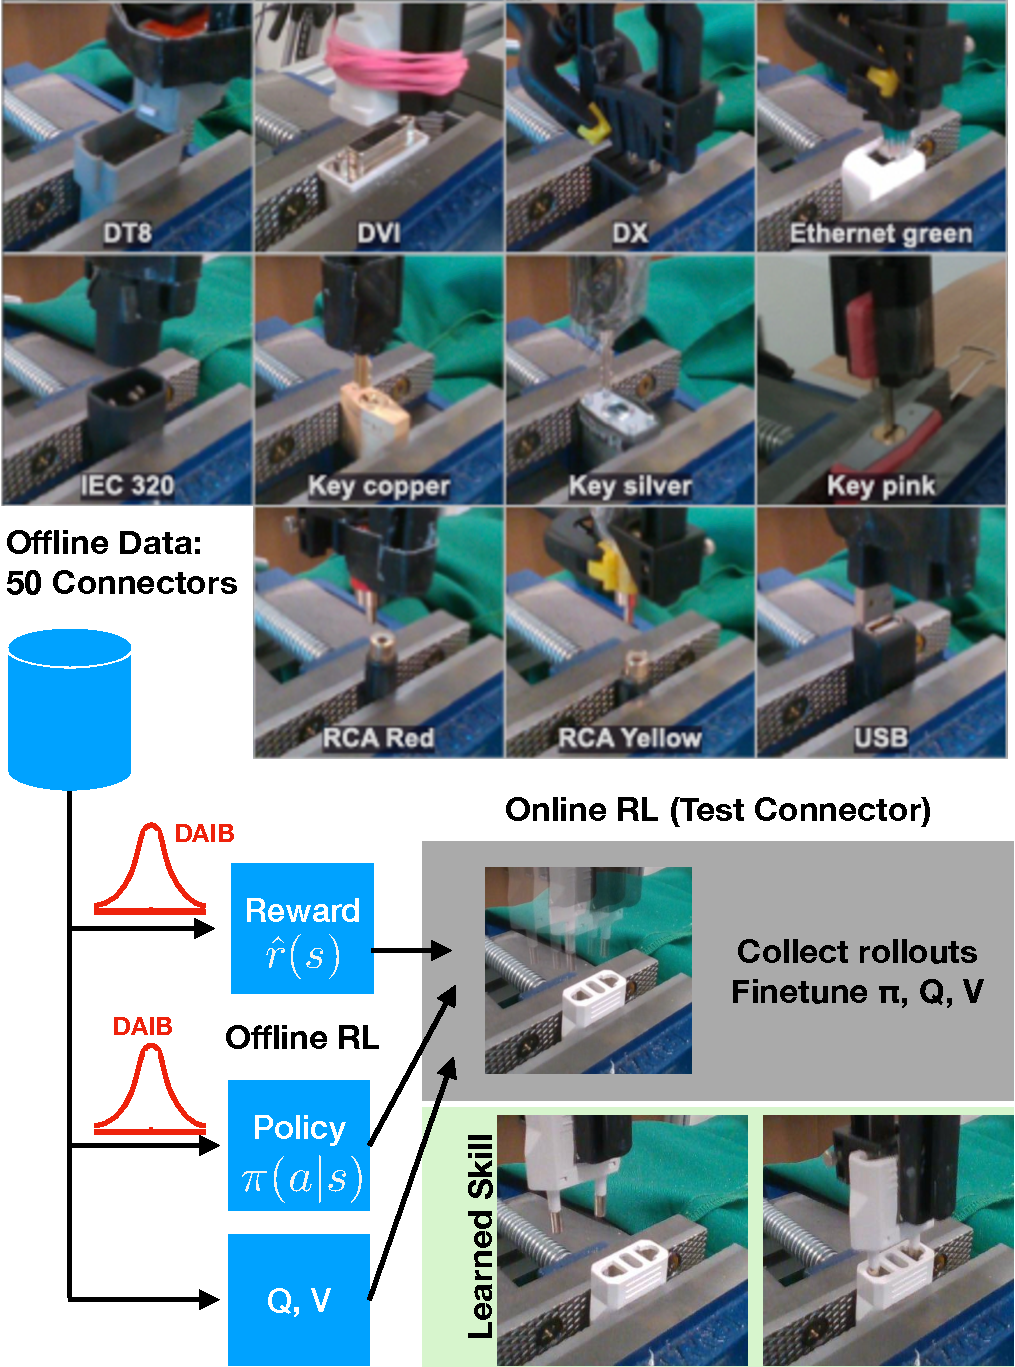
\includegraphics[width=0.99\textwidth]{imgs/fig1_v2-crop.pdf}
    \end{subfigure}

    \caption{We use offline reinforcement learning on insertion data on a diverse set of connectors (left) followed by online finetuning to solve a connector-socket insertion task from vision on a previously unseen connector (right).}
%%SL.6.8: Great to have a page 1 figure like this, but it would be good if it actually provides a diagram illustrating the method at a high level, rather than just some robot pictures (though it's good of course to show lots of connectors). I also found the photos to be extremely hard to parse. It's good that they're diverse, but I can barely see the connector in most of them.
    \label{fig:fig1}
    % \vspace{-0.5cm}
% \end{wrapfigure}
\end{figure}

We study this problem in the setting of learning a policy from vision for performing industrial insertion tasks.
This family of assembly tasks, including plugging in connectors into sockets, screwdrivers into screw intrusions, setting screws, and so on, are found in many stages of manufacturing.
%%SL.6.8: Good, but don't overclaim! The paper is not doing "screwdrivers into screw intrusions".
%%AVN.7.18 we do have data including hex screwdrivers etc.
When automated in factories today, these tasks are done by robots with specialized control algorithms that rely on precise localization of the socket location.
% In many instances, humans are required to do these tasks instead because the environment cannot be carefully controlled.
% For robots to perform these insertion tasks in industrial and warehouse settings with less human supervision, or in unstructured environments such as homes, they cannot rely on highly accurate state information of the external world (ie. the socket position).
%%SL.6.8: I really don't think that most people will think "state information" = socket location. The first few times I read this, I was sure "state information" meant robot state (i.e., joint angles). Maybe use a different terminology?
%%AVN.7.18 made more explicit
For robots to perform these insertion tasks in industrial and warehouse settings with less human supervision, or in unstructured environments such as homes, they must rely on highly accurate state information of the external world (ie. socket position and in-hand pose estimation).
But such state estimation, using either machine learning or computer vision approaches, is brittle on unseen connectors.
To solve the general problem of inserting a novel connector, one promising solution is to generalize previously collected experience of connector insertion to learn a policy to insert connectors from vision.
%%SL.6.8: The above doesn't really explain the problem. Is the problem to insert one connector? "generalize" to what?
% Importantly, collecting very broad datasets in this domain for visual generalization is a challenge because collecting data for each connector requires significant setup and supervision, so the quantity of prior experience is limited.
%%SL.6.8: but isn't collecting such a dataset precisely what this paper does?
% Errors could be introduced in localizing the socket, grasping the connector, and so on, which can make state-based algorithms brittle.
% Instead, if robots had semantic visual understanding of connector-socket insertion tasks and feedback visuomotor control policies to accomplish them, a much broader array of these tasks could be automated.
Among these tasks, there is enough variability to require generalization and adaptation, but also enough internal structural regularity that we expect transfer between different connectors.
We first collected a large offline dataset with insertion data of \numconnectors{} connectors across 2 robots and diverse backgrounds with actions, images, and sparse reward labels.
How can a robot generalize from vision to test connectors in this setting, utilizing offline reinforcement learning from this data to enable active online fine-tuning on a new connector?
%%SL.6.8: These last two sentences are great! But it would be good for the rest of the paragraph to be improved to lead up to that

% One of the main observations we make in this work is that, with a suitable representation learning and domain adaptation approach, it can be significantly easier for the reward function to generalize to a new but structurally similar task (e.g., inserting a new type of connector) than for the policy. This means that a learned reward function can be used to facilitate the finetuning of the robot's policy in situations where the policy fails to generalize in zero shot, but the reward function generalizes successfully.

The key insight is that we need to (1) find common structure between domains while preserving important domain-specific information and (2) adapt to new tasks quickly with online data if the zero-shot solution is not sufficient.
%%SL.6.8: The above sentence reads very well!
For finding common structure while preserving important domain-specific information, we propose a split representation that combines domain adversarial neural networks~\cite{ganin2016domainadversarial} for domain invariance and a variational information bottleneck~\cite{alemi2017vib}
for controlling the flow of domain-specific information.
This representation, which we call \methodname{} (\methodabbrv) is used first for learning a robust reward function to detect successful insertions for an unseen connector.
% We propose to use an auxiliary contrastive representation learning objective that aligns disparate domains to address this issue.
%%SL.5.25: not quite clear what "disparate domains" refers to here
% To learn low-dimensional representations from large (160x160) image input for sample-efficient RL, we use the standard self-contrastive learning objective with data augmentations.
%%SL.5.25: that doesn't sound like a contribution, it kind of just sounds like we use a thing that already exists
%%AVN.6.2 Rephrased to emphasize the new thing (but agreed it is not super novel)
% To align data from diverse domains, we propose to use a self-contrastive learning objective, contrastive domain alignment (CDA),
%%SL.6.8: is this an existing algorithm? if so, cite it; writing wise, maybe add a bit of motivation for why we do this?
% with data augmentations additionally treating all observations with positive rewards (i.e., images of successful insertions) as positives.
%%SL.6.8: The above sounds good (if a bit laundry-list), but the stuff below doesn't follow logically from the above. Should these be separate paragraphs? Feels like there is a very sudden jump right here.
Next, we use the representation for training a reward function, policy, and Q function that can also generalize to new connectors, by modifying implicit Q-learning (IQL), an offline RL algorithm amenable to online fine-tuning, to use \methodabbrv{}.
Then, during online finetuning, this auxiliary objective can be used in combination with online RL to enable fast learning of novel connectors.
% For finetuning without external state information, we require an accurate reward model that generalizes.
%%SL.6.8: The first half of the above paragraph (about the contrastive thing) reads well, but the stuff afterwards (To train models...) again is a bit incoherent, with sentences not following logically from one another. Probably that should be a separate paragraph, but it likely also needs to be somewhat rewritten to flow more smoothly
%%AVN.7.18 rewritten and separated into two paragraphs


% Contributions
We present two major contributions.
First, we propose a novel representation learning method that allows better generalization of policies and reward functions.
This enables fast finetuning of vision-based IQL policies on a new domain. 
%%SL.6.8: nothing in the above sentences talks about offline training on multiple connectors... kind of weird
Second, we present a system based off of this representation learning method to insert connectors robustly from vision without the need of accurate socket localization,
%%SL.6.8: see above comment about "state information"
both for observations and rewards. We outperform a regression-based baseline on the same dataset that attempts to localize the socket.
We show that new tasks can be fine-tuned within 200 trials, given our dataset of off-policy data from Y prior tasks of Z trajectories.
This system allows us to finetune IQL to a test connector, increasing performance significantly over the offline performance.
Our dataset of robotic insertion of \numconnectors{} connectors, as well as pretrained features and reward models will be made public at <URL>.


% %%%%%%%%%%%% OLD INTRO

% % Models that are pre-trained on broad, diverse datasets and can be fine-tuned to specific problems have driven recent progress in vision and NLP~\cite{krizhevsky2012imagenet, devlin2019bert}.
% % Perhaps the same kind of generalization could be attained in robotics by collecting broad datasets for particular classes of tasks and training general policies from these datasets that can perform these tasks in diverse settings and with varied objects.
% % But in robotics, collecting diverse data is itself a challenge, and robotics datasets are often are still limited to one or few robots, performing tasks in a few distinct domains with highly correlated background, objects, and tasks within a domain~\cite{ebert2021bridge, dasari2019robonet}.
% % % However, in robotics, this is a difficult challenge due to hardware, setup, and supervision costs of collecting diverse data.
% % %%SL.6.8: I don't understand the above sentence -- what is the challenge due to "hardware, setup" and what supervision cost are you talking about? I would suggest just rewriting it, as right now it kind of reads like a "generic" motivation (and one that is somewhat logically inconsistent)
% % % Because of this, robotics datasets are often are still limited to one or few robots, performing tasks in a few distinct domains with highly correlated background, objects, and tasks within a domain~\cite{ebert2021bridge, dasari2019robonet}.
% % %%SL.6.8: kind of implies that a contribution of this paper is to collect a broader dataset, which is not actually the case
% % Generalizing to a new domain from prior data of few domains is difficult, so in robotics we need more than the paradigm of learning from offline datasets and generalizing zero-shot.
% % On the other hand, robotics offers a unique opportunity in being able to interact online in the test environment and collect new data.
% % The online data can provide extra signal for adapting representations to perform well in the new domain.
% % Instead of expecting perfect zero-shot generalization, if we could learn from offline datasets containing few domains, then fine-tune on a task in a new domain, it would greatly broaden applicability of learning-based robotics.
% % %%SL.6.8: I would recommend rewriting the above paragraph. I do think it has the right idea, but the sentences do not follow each other in a logical manner. Try to think of the main idea you want to get across and make sure that each sentence builds on the previous one and there is a clear logical progression.

% Models that generalize from training on broad, diverse datasets have driven recent progress in vision and NLP~\cite{krizhevsky2012imagenet, devlin2019bert}.
% We hope to do the same in robotics with offline reinforcement learning, but zero-shot generalization of policies may not always be possible.
% Since robotics datasets are often are still limited to one or few robots, performing tasks in a few distinct domains with highly correlated background, objects, and tasks within a domain~\cite{ebert2021bridge, dasari2019robonet}, generalizing to new tasks and new domains can be very challenging.
% But zero-shot generalization may also not always be necessary.
% If whenever the policy does not generalize to an unseen task, reward functions and value functions generalize instead, we can utilize these in order to actively practice the task to improve the policy, greatly broadening applicability of learning-based robotics.

% We study this problem in the setting of learning a policy from vision for performing industrial insertion tasks.
% This family of assembly tasks, including plugging in connectors into sockets, screwdrivers into screw intrusions, setting screws, and so on, are found in many stages of manufacturing.
% %%SL.6.8: Good, but don't overclaim! The paper is not doing "screwdrivers into screw intrusions".
% %%AVN.7.18 we do have data including hex screwdrivers etc.
% When automated in factories today, these tasks are done by robots with specialized control algorithms that rely on precise localization of the socket location.
% % In many instances, humans are required to do these tasks instead because the environment cannot be carefully controlled.
% % For robots to perform these insertion tasks in industrial and warehouse settings with less human supervision, or in unstructured environments such as homes, they cannot rely on highly accurate state information of the external world (ie. the socket position).
% %%SL.6.8: I really don't think that most people will think "state information" = socket location. The first few times I read this, I was sure "state information" meant robot state (i.e., joint angles). Maybe use a different terminology?
% %%AVN.7.18 made more explicit
% For robots to perform these insertion tasks in industrial and warehouse settings with less human supervision, or in unstructured environments such as homes, they must rely on highly accurate state information of the external world (ie. socket position and in-hand pose estimation).
% But such state estimation, using either machine learning or computer vision approaches, is brittle on unseen connectors.
% To solve the general problem of inserting a novel connector, one promising solution is to generalize previously collected experience of connector insertion to learn a policy to insert connectors from vision.
% %%SL.6.8: The above doesn't really explain the problem. Is the problem to insert one connector? "generalize" to what?
% % Importantly, collecting very broad datasets in this domain for visual generalization is a challenge because collecting data for each connector requires significant setup and supervision, so the quantity of prior experience is limited.
% %%SL.6.8: but isn't collecting such a dataset precisely what this paper does?
% % Errors could be introduced in localizing the socket, grasping the connector, and so on, which can make state-based algorithms brittle.
% % Instead, if robots had semantic visual understanding of connector-socket insertion tasks and feedback visuomotor control policies to accomplish them, a much broader array of these tasks could be automated.
% Among these tasks, there is enough variability to require generalization and adaptation, but also enough internal structural regularity that we expect transfer between different connectors.
% How can a robot generalize from vision to test connectors in this setting, utilizing offline reinforcement learning but also active online fine-tuning?
% %%SL.6.8: These last two sentences are great! But it would be good for the rest of the paragraph to be improved to lead up to that

% The key insight is that we need to (1) find common structure between domains while preserving important domain-specific information and (2) adapt to new tasks quickly with online data if the zero-shot solution is not sufficient.
% %%SL.6.8: The above sentence reads very well!
% For finding common structure while preserving important domain-specific information, we propose a split representation that combines domain adversarial neural networks~\cite{ganin2016domainadversarial} for domain invariance and a variational information bottleneck~\cite{alemi2017vib}
% for controlling the flow of domain-specific information.
% This representation, which we call \methodname{} (\methodabbrv) is used first for learning a robust reward function to detect successful insertions for an unseen connector.
% % We propose to use an auxiliary contrastive representation learning objective that aligns disparate domains to address this issue.
% %%SL.5.25: not quite clear what "disparate domains" refers to here
% % To learn low-dimensional representations from large (160x160) image input for sample-efficient RL, we use the standard self-contrastive learning objective with data augmentations.
% %%SL.5.25: that doesn't sound like a contribution, it kind of just sounds like we use a thing that already exists
% %%AVN.6.2 Rephrased to emphasize the new thing (but agreed it is not super novel)
% % To align data from diverse domains, we propose to use a self-contrastive learning objective, contrastive domain alignment (CDA),
% %%SL.6.8: is this an existing algorithm? if so, cite it; writing wise, maybe add a bit of motivation for why we do this?
% % with data augmentations additionally treating all observations with positive rewards (i.e., images of successful insertions) as positives.
% %%SL.6.8: The above sounds good (if a bit laundry-list), but the stuff below doesn't follow logically from the above. Should these be separate paragraphs? Feels like there is a very sudden jump right here.
% Next, we use the representation for training a reward function, policy, and Q function that can also generalize to new connectors, by modifying implicit Q-learning (IQL), an offline RL algorithm amenable to online fine-tuning, to use \methodabbrv{}.
% Then, during online finetuning, this auxiliary objective can be used in combination with online RL to enable fast learning of novel connectors.
% % For finetuning without external state information, we require an accurate reward model that generalizes.
% %%SL.6.8: The first half of the above paragraph (about the contrastive thing) reads well, but the stuff afterwards (To train models...) again is a bit incoherent, with sentences not following logically from one another. Probably that should be a separate paragraph, but it likely also needs to be somewhat rewritten to flow more smoothly
% %%AVN.7.18 rewritten and separated into two paragraphs

% \begin{figure}[b]
%     \centering
%     \begin{subfigure}[b]{0.9\linewidth}
%         \center
%         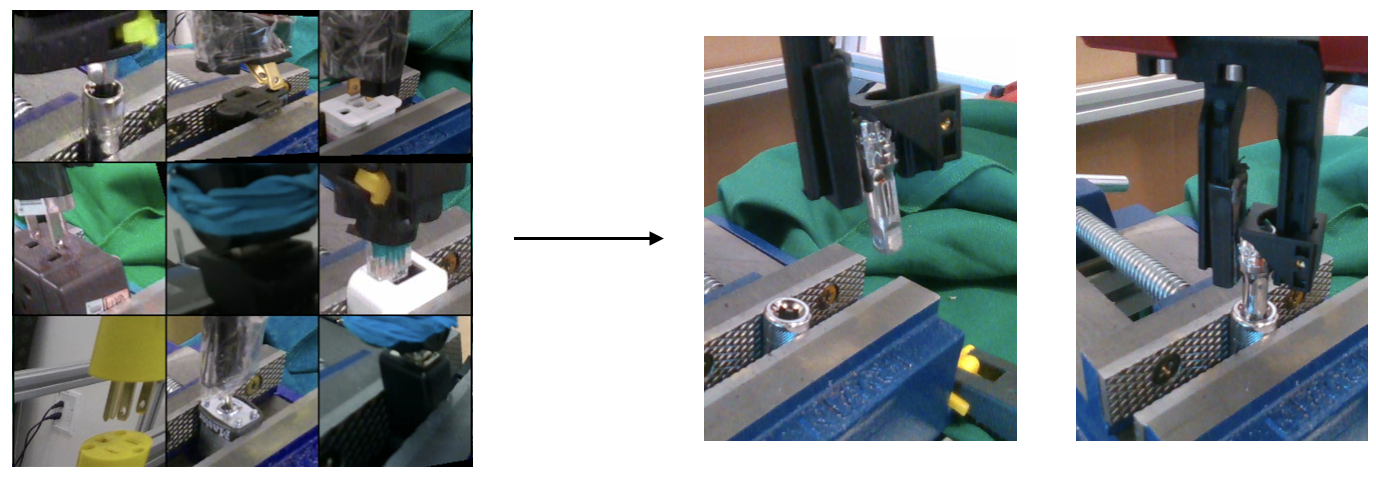
\includegraphics[width=0.9\textwidth]{imgs/fig1.png}
%     \end{subfigure}

%     \caption{We use offline reinforcement learning on insertion data on a diverse set of connectors (left) followed by online finetuning to solve a connector-socket insertion task from vision on a previously unseen connector (right).}
% %%SL.6.8: Great to have a page 1 figure like this, but it would be good if it actually provides a diagram illustrating the method at a high level, rather than just some robot pictures (though it's good of course to show lots of connectors). I also found the photos to be extremely hard to parse. It's good that they're diverse, but I can barely see the connector in most of them.
%     \label{fig:fig1}
%     \vspace{-0.5cm}
% % \end{wrapfigure}
% \end{figure}

% To train models to generalize to test connectors, we first collected a large offline dataset with insertion data of \numconnectors{} connectors across 2 robots and diverse backgrounds with actions, images, and sparse reward labels.
% We first demonstrate that with the \methodabbrv{} representation, our reward function on a test connector is more accurate than alternative representation learning methods.
% We show that the \methodabbrv{} representation learning objective helps train policies that generalize better from offline training to an unseen connector.
% Finally, we show that fine-tuning this policy with rewards and Q-functions that generalize with the \methodabbrv{} representation significantly improve performance.
% %%SL.6.8: definitely doesn't belong in the same paragraph -- don't mix together the summary/motivation of the technical method and the results like that
% %%AVN.7.18: it is split now

% % Contributions
% We present two major contributions.
% First, we propose a novel representation learning method that allows better generalization of policies and reward functions.
% This enables fast finetuning of vision-based IQL policies on a new domain. 
% %%SL.6.8: nothing in the above sentences talks about offline training on multiple connectors... kind of weird
% Second, we present a system based off of this representation learning method to insert connectors robustly from vision without the need of accurate socket localization,
% %%SL.6.8: see above comment about "state information"
% both for observations and rewards. We outperform a regression-based baseline on the same dataset that attempts to localize the socket.
% We show that new tasks can be fine-tuned within 200 trials, given our dataset of off-policy data from Y prior tasks of Z trajectories.
% This system allows us to finetune IQL to a test connector, increasing performance significantly over the offline performance.
% Our dataset of robotic insertion of \numconnectors{} connectors, as well as pretrained features and reward models will be made public at <URL>.

% %%% OLD INTRO %%%%%%%%%%%

% We face several challenges .
% First, no existing public dataset contains data of diverse insertion tasks with image input.
% %%SL.6.2: I think the bar for presenting a public dataset that people can use is much higher than what this paper is likely to accomplish, so I would not recommend claiming that the release of a public (reusable) dataset is one of the contributions unless you are prepared to put in the work to make it usable and convince the readers of this (which I don't think is entirely realistic in the remaining time). If we're not claiming that, then we shouldn't motivate from this perspective.
% We collected a large offline dataset with insertion data of \numconnectors connectors across 2 robots and diverse backgrounds with actions, images, and clean sparse reward labels.
% %%SL.6.2: Before talking about what we do, we should motivate the approach.
% We use this data for offline RL but release it publicly so it can be used by others for domain adaptation, dynamics understanding of contact-rich tasks, or finetuning to their own insertion problems.
% %%SL.6.2: Good to note we release it, but not so prominently (because you won't be able to convince readers that this is useful)
% Second, we utilize offline RL to learn policies on this data, but it may not generalize zero-shot to all potential insertion tasks.
% %%SL.6.2: This needs to be motivated earlier.
% Instead of relying solely on zero-shot generalization, we can also fine-tune the policy with additional data collected online on the target connector.
% For finetuning, we need an accurate reward function, since we cannot rely on state information for rewards either.
% Finally, since there is a relatively high setup cost of collecting data on individual connectors, the dataset is highly correlated and only contains around \numconnectors visually distinct settings.
% All these learned models - policies, value functions, and rewards, they need to generalize from a small number of individual domains (connectors, robots, and backgrounds) to a new domain.

% What does it take to fine-tune on test environments?
% First, to improve in a test environment we need not only a policy that generalizes but also a reward model. 
% First of all we need an accurate reward model.
% Second, we need algorithms that can train offline and finetune.
% Third, we need generalization of .

% Describe domain adaptation representation learning method

% Contributions

% The success of deep learning
% Deep learning for vision-based robotics
% But its hard to collect robotics in data
% For example, consider industrial insertion
% The idea is best evaluated on a family of tasks where there is enough variability to require generalization and adaptation, but also considerable internal structural regularity so that we have reason to expect things to generalize.
% Consider learning a policy from vision for performing industrial insertion tasks, a frequently encountered problem in manufacturing.
% Few-domain datasets
% Zero-shot generalization is hard
% Instead we can fine-tune

% What does it take to fine-tune?
% First we need rewards
% We need algorithms that can train offline and finetune
% We also need generalization


% \section{Introduction}

% % what is the problem
% Industrial insertion is a frequently encountered problem in manufacturing. This family of assembly tasks, including plugging in connectors into sockets, screwdrivers into screw intrusions, setting screws, and so on, are found in many stages of manufacturing.
% When automated in factories today, these tasks are done by robots with specialized control algorithms which rely on precise state information of the socket location and carefully managed physical setups, such as assembly lines, to succeed at the task.
% In many instances, humans are required to do these tasks instead because the environment cannot be carefully controlled.
% For robots to perform these insertion tasks in industrial and warehouse settings with less human supervision, or in unstructured environments such as homes, they cannot rely on highly accurate state information.
% Errors could be introduced in localizing the socket, grasping the connector, and so on, which can make state-based algorithms brittle.
% Instead, if robots had semantic visual understanding of connector-socket insertion tasks and feedback visuomotor control policies to accomplish them, a much broader array of these tasks could be automated.
% %%SL.6.2: I think the introduction still has the same problem I pointed out before: it is motivated from two seemingly unrelated perspectives, both as an application-centric paper focusing on industrial insertion, and as a study of offline RL. We could discuss how to best motivate it, but I'm not sure if a purely insertion-centric motivation will be that successful, because I think if people look at this alongside other works on industrial insertion, I doubt the method will stand out in terms of how well it works for insertion in particular. But the generality of the approach could be more compelling. Perhaps a motivation that discusses the broader, more general motivation with industrial insertion as an application area would work better? E.g., one way you could motivate this is to talk about how the main idea is best evaluated on a family of tasks where there is enough variability to require generalization and adaptation, but also considerable internal structural regularity so that we have reason to expect things to generalize.

% Reinforcement learning from offline data is a promising approach to learn robust feedback control policies from vision that generalize to new connectors and errors in grasping and socket localization.
% %%SL.6.2: But the method is not just about RL from offline data?
% However, there are many remaining challenges applying RL in this setting.
% First, no existing public dataset contains data of diverse insertion tasks with image input.
% %%SL.6.2: I think the bar for presenting a public dataset that people can use is much higher than what this paper is likely to accomplish, so I would not recommend claiming that the release of a public (reusable) dataset is one of the contributions unless you are prepared to put in the work to make it usable and convince the readers of this (which I don't think is entirely realistic in the remaining time). If we're not claiming that, then we shouldn't motivate from this perspective.
% We collected a large offline dataset with insertion data of \numconnectors connectors across 2 robots and diverse backgrounds with actions, images, and clean sparse reward labels.
% %%SL.6.2: Before talking about what we do, we should motivate the approach.
% We use this data for offline RL but release it publicly so it can be used by others for domain adaptation, dynamics understanding of contact-rich tasks, or finetuning to their own insertion problems.
% %%SL.6.2: Good to note we release it, but not so prominently (because you won't be able to convince readers that this is useful)
% Second, we utilize offline RL to learn policies on this data, but it may not generalize zero-shot to all potential insertion tasks.
% %%SL.6.2: This needs to be motivated earlier.
% Instead of relying solely on zero-shot generalization, we can also fine-tune the policy with additional data collected online on the target connector.
% For finetuning, we need an accurate reward function, since we cannot rely on state information for rewards either.
% Finally, since there is a relatively high setup cost of collecting data on individual connectors, the dataset is highly correlated and only contains around \numconnectors visually distinct settings.
% All these learned models - policies, value functions, and rewards, they need to generalize from a small number of individual domains (connectors, robots, and backgrounds) to a new domain.
% %%SL.6.2: I recommend rewriting this paragraph to motivate the approach, not clutter it with talk about releasing a dataset (the dataset is not going to be useful to anyone but us anyway, so it's hard for readers to see this as a serious contribution), and motivate why we do particular things before stating what they are

% % why is it hard
% % While prior methods have addressed connector insertion from vision, they assume relatively accurate state information with $\pm2\text{mm}$. In contrast, we solve tasks from vision with the connector starting $\pm2\text{cm}$ away from the socket. In this setting, simply doing structured exploration is not enough: vision is required.

% %%SL.6.2: The content of this paragraph doesn't seem to be motivated at all in the preceding discussion
% % main components of our approach
% We propose to use an auxiliary contrastive representation learning objective that aligns disparate domains to address this issue.
% %%SL.5.25: not quite clear what "disparate domains" refers to here
% % To learn low-dimensional representations from large (160x160) image input for sample-efficient RL, we use the standard self-contrastive learning objective with data augmentations.
% %%SL.5.25: that doesn't sound like a contribution, it kind of just sounds like we use a thing that already exists
% %%AVN.6.2 Rephrased to emphasize the new thing (but agreed it is not super novel)
% To align data from diverse domains, we use a self-contrastive learning objective with data augmentations additionally treat all observations with positive rewards (i.e., images of successful insertions) as positives.
% We first show that this representation learning objective helps the reward and policy generalize better to an unseen connector. 
% Then, during online finetuning, this auxiliary objective can be used in combination with online RL with a high number of gradient updates per environment step to stabilize and accelerate learning.

% % Contributions
% We present three key contributions.
% First, we propose a novel representation learning method that allows better generalization of policies and reward functions.
% This enables fast finetuning of vision-based IQL policies on a new domain. 
% %%SL.5.25: this is not a complete sentence! also, you said before it's a standard method, but now it's a novel method?
% Second, we present a system based off of this representation learning method to insert robustly from vision without the need of state information, both for observations and rewards.
% We show that new tasks can be learned within X trials, given our dataset of off-policy data from Y prior tasks of Z trajectories.
% This system allows us to finetune a connector with grasping in the loop {\color{blue}
% (assuming this works.)}.
% % Using this system, we collected high-quality insertion data on Y connectors.
% %%SL.5.25: why is this important?
% %%AVN.6.2. I think the dataset is an important contribution; however it looks like it probably will not be collected in an on-policy way. I added discussion of the dataset above though
% Our third contribution is to release a dataset for robotic insertion connectors, as well as pretrained features and reward models.
% %%SL.6.2: really don't think this will work
% %%SL.5.25: this kind of comes out of nowhere, wasn't mentioned or discussed before; if the dataset is one of the contributions, you would need to actually discuss it in detail and explain how it's useful to people (you could just remark that we release the dataset without claiming that it is one of the contributions, if you don't want to deal with this problem)
% Our dataset will be made public at <URL>.

% \section{Introduction}

% Models that are pre-trained on broad datasets and can be fine-tuned to specific problems, sometimes called ``foundation models''
% %%SL.5.25: Kind of a matter of preference, but I'm not big fan of this (re)branding of pretrained models. I suspect it's easy enough to get people to understand what you mean without it.
% have driven recent progress in vision and NLP.
% For instance, bidirection encoders from transformers (BERT) ~\cite{devlin2019bert} pretrained on large language datasets (100Ms of sentences) is now the standard starting point for fine-tuning to language models on custom language tasks and on custom data of much smaller size (10,000s of sentences).
% This type of pretraining capability enables machine learning to be used to solve more bespoke problems, greatly widening the applicability of ML methods to real-world applications.
% Similarly, robotics applications are often narrow, so the ability to utilize broad prior data but fine-tune on a specific task would be extremely valuable.
% %%SL.5.25 I think this is a great story, but I'm just not sure this story really makes sense for the present paper. We are not really training the system on particularly broad or large datasets compared to other work in robotic learning (and arguably many prior papers have used much larger and much broader datasets), so it might kind of rub people the wrong way to scope the claims around this. Generally, people expect that the claims will follow from the motivation, so if the motivation is that effective generalization can be attained from broad and diverse datasets and large models, people will expect to see the paper make a contribution in demonstrating this (moreso than prior papers), which I don't think is what this paper really does.

% % What is the problem
% % visual insertion to recover from misgrasps
% One problem where the recipe of pretraining followed online finetuning could be very impactful is in solving industrial insertion tasks from vision.
% Industrial insertion tasks, such as inserting plugs in sockets and setting screws, are automated in factories today with specialized control algorithms.
% %%SL.5.25: I think the current story here is pretty unfocused, it kind of comes across as though the paper can't decide whether it's about an application (insertion) or about a technical concept (offline training + finetuning). The paper really needs to have one central problem, one central thesis, it's exceptionally difficult to tell a compelling story without committing to one vision.
% These algorithms depend on precise motions and proprioceptive information, which can make them susceptible to failing in high-variance conditions, such as when there is a misgrasp of a connector to insert into a socket.
% %%SL.5.25: Above doesn't quite make sense to me ("misgrasp of a connector to insert")
% Instead, if the insertion policy could perform visual feedback, it could robustly handle such variation and broaden the potential use of robots in industrial settings.
% In this paper, we explore training vision policies that perform robust visual servoing in the face of significant variation ($\pm$2cm translation and $\pm 5^{\circ}$ rotation in each axis) by training implicit
% %%SL.5.25: we explore training ... by training
% Q-learning (IQL) on data from 50+ connectors.
% The policy can generalize to a new connector and finetune to improve performance.

% % Why is it interesting and important

% % Why is it hard?
% However, as we show in our experiments, offline RL followed by online finetuning of a large convolutional neural network policy using IQL does not work out of the box.
% The finetuning setting ought to offer significant advantages over offline RL, as instead of generalizing zero-shot to a new setting, the policy gets to experience the new setting directly.
% {
% \color{blue}
% (We have some evidence but not completely confident of the following.)
% }
% But in practice, online finetuning the entire policy destroys convolutional layers due to overestimated advantages on online data, while freezing the convolutional layers leads to slow learning.
% We need an offline and online representation learning objective that can quickly adapt the representation on a small amount of online data for RL.
% %%SL.5.25: There are some major issues in this paragraph. First, this kind of comes out of nowhere (i.e., this problem is not motivated by the original problem statement). Second, it's not clear how this issue is specific to the problem you are considering -- it comes across as just a general problem that comes up when training neural nets with deep RL. Perhaps the thing to do would be to somewhat reorient the beginning of the intro to motivate representation learning, so that you can steer the discussion in this direciton from the start, making it clear how representation learning ties into the offline -> online problem statement and into robotic manipulation more generally.

% Our solution
% {
% \color{blue}
% (Proposed fix, haven't seen gains from this yet.)
% }
% We propose to use an auxiliary contrastive representation learning objective that aligns disparate domains to address this issue.
% %%SL.5.25: not quite clear what "disparate domains" refers to here
% To learn low-dimensional representations from large (160x160) image input for sample-efficient RL, we use the standard self-contrastive learning objective with data augmentations.
% %%SL.5.25: that doesn't sound like a contribution, it kind of just sounds like we use a thing that already exists
% To align data from diverse domains, we additionally treat all observations with positive rewards (i.e., images of successful insertions) as positives.
% During online finetuning, this auxiliary objective can be used in combination with online RL with a high number of gradient updates per environment step to stabilize and accelerate learning.

% % Contributions
% We present three key contributions.
% First, a novel representation learning method that enables fast finetuning of vision-based IQL policies on a new domain. 
% %%SL.5.25: this is not a complete sentence! also, you said before it's a standard method, but now it's a novel method?
% Second, a system based off of this representation learning method to insert robustly from vision without the need of state information, both for observations and rewards.
% We show that new tasks can be learned within X trials, given our dataset of off-policy data from Y prior tasks of Z trajectories.
% This system allows us to finetune a connector with grasping in the loop {\color{blue}
% (assuming this works.)}.
% Using this system, we collected high-quality insertion data on Y connectors.
% %%SL.5.25: why is this important?
% Our third contribution is to release a dataset for robotic insertion connectors, as well as pretrained features and reward models.
% %%SL.5.25: this kind of comes out of nowhere, wasn't mentioned or discussed before; if the dataset is one of the contributions, you would need to actually discuss it in detail and explain how it's useful to people (you could just remark that we release the dataset without claiming that it is one of the contributions, if you don't want to deal with this problem)
% Our dataset will be made public at <URL>.

\section{Related Work}

%%SL.6.2: Remember that the organization of the related work should reflect the contribution of the paper. It makes sense to start by talking about reinforcement learning for robotics if we position the paper such that this is the core area of the paper. But right now the intro positions the paper first and foremost as a contribution in industrial insertion, making this rather incongruent.

Our work proposes a system for finetuning an offline reinforcement learning policy on new tasks in realistic industrial insertion scenarios, using a novel representation learning method for generalization to a test domain. In this section, we discuss prior work on reinforcement learning, industrial insertion, and representation learning.
%%SL.6.8: could probably cut the above para if we're short on space or replace with one sentence; you could also cut the paragraph headings and start the first para with a transition sentence (in fact the sentence is already a good transition...)

\textbf{Reinforcement learning for robotics.}
% General RL, offline RL for robotics, online finetuning
Reinforcement learning has been applied successfully to a variety of robotics tasks in both manipulation~\cite{peters2008baseball, kober2008mp,deisenroth2011pilco, levine2016gps, levine2017grasping, zhu2019hands} and locomotion~\cite{giusti15trails, nakanishi2004bipedlfd, kalakrishnan09terraintemplates} settings.
%%SL.6.2: not sure what the significance of "model-based control" here is (and most of those papers don't use it, unless you consider PD control "model-based", which it isn't)
To utilize offline datasets with diverse data in robotics, algorithms developed for offline reinforcement learning~\cite{fujimoto19bcq, kumar2020cql, nair2020awac, wu2019brac} have been studied in the robotics setting~\cite{singh2020cog, singh2020parrot, chebotar2021actionable, kalashnikov2021mtopt, kumar2021workflow}.
%%SL.5.25: need to explain the difference (there are many works on offline pretraining now)
A subset of offline RL algorithms are amenable to finetuning ~\cite{nair2020awac,villaflor2020finetuning, meng2021starcraft, lee2021finetuning,kostrikov2021iql}.
Our work builds on the direction of offline pretraining followed by online finetuning in robotics.
But beyond this line of work, we focus on finetuning from visual input in realistic settings with multiple domains and without ground truth reward functions at test time.

% Self-supervised RL, how this paper is different
In this respect, our work is closest to prior work on self-supervised RL that does not assume an external reward function and instead learns it from data.
One class of self-supervised reinforcement learning methods uses goal-conditioned RL with self-supervised rewards~\cite{kaelbling1993goals, schaul2015uva, Baranes2012, andrychowicz2017her, nair2018rig, nachum2018hiro, held2018goalgan, Pere2018, wadefarley2019discern, pong2020skewfit, khazatsky2021val}.
While general, this class of methods is a poor fit for industrial insertion, as high precision is required in both the policy and in evaluating rewards.
Instead, we train a domain generalizing reward classifier from prior data.
Prior methods have used learned rewards~\cite{pong2022smac} and classifier rewards have been proposed as a scalable solution for robotics tasks previously~\cite{fu2018vice, singh2019raq}.
However, learned rewards have not been shown to be useful for fine-tuning in novel robotic domains previously.
Because we focus on applying offline RL and fine-tuning from vision in the industrial insertion setting in this work, few-domain generalization of the reward function is vital for our method to work in practice.
% This setting poses unique challenges due to the need to generalize from few domains, which we address via representation learning.

% Model-free deep reinforcement learning algorithms in particular have shown human-level or superhuman performance using rich observations on sequential decision making tasks such as games~\cite{mnih2013atari, silver2016alphago}.
%%SL.5.25: what does this have to do with the previous sentence about robotics tasks?
%%AVN.6.2. reordered, to make the point that model-free RL for robotics is a good idea if done offline
%%SL.6.2: It still doesn't make sense to me -- why start a paragraph on RL for robotics with a sentence about RL that has nothing to do with robotics? It might kind of make sense if the sentence was about foundational work in RL, but that's not what is cited either.
% However, these algorithms have usually been trained from scratch,
%%SL.6.2: nitpick -- it's not the algorithms that are trained, it's policies that are trained via those algorithms
% which can be prohibitive for real-world robotics.
%%SL.6.2: there are plenty of papers on training robotic policies with RL from scratch, so obviously it is not prohibitive (and authors of those papers are likely to be reviewing this paper, and will reject it for deceptive discussion of related work)
% Reinforcement learning has been applied successfully to a variety of robotics tasks in both manipulation~\cite{peters2008baseball, kober2008mp,deisenroth2011pilco, levine2016gps, levine2017grasping} and locomotion~\cite{giusti15trails, nakanishi2004bipedlfd, kalakrishnan09terraintemplates} settings.
% %%SL.6.2: not sure what the significance of "model-based control" here is (and most of those papers don't use it, unless you consider PD control "model-based", which it isn't)
% To utilize offline datasets with diverse data, specialized algorithms have been developed~\cite{chebotar2021actionable, kalashnikov2021mtopt, nair2020awac}.
% %%SL.5.25: need to explain the difference (there are many works on offline pretraining now)
% In this work, we focus on applying offline RL and fine-tuning from vision in the industrial insertion setting.
% This setting poses unique challenges due to the need to generalize from few domains, which we address via representation learning.
%%SL.6.2: This is a really weak paragraph for related work. Can you discuss the most closely related stuff and explain how this paper is different? The above paragraph says more or less nothing about the distinction between the prior work and this paper.
%%AVN.6.8: if representation learning is the main thing, is there a need to communicate a distinction between this and prior RL papers (without represnetation learning) if it is covered in the previous paragraph?

\textbf{Robotic insertion.} Prior work has discussed reinforcement learning for robotic insertion.
Initial work in this direction focuses on learning
%%TODO cite the older work before learning
%%SL.6.2: initial work in this direction has nothing to do with learning and is much older than this
for a single connector from ground-truth state information~\cite{lian2021insertionbenchmark, johannink18residualrl, schoettler2019insertion}.
In this case, the RL algorithm must learn to navigate the specific dynamics of the single connector, but does not generalize across connectors.
More recent work has considered using meta-learning to generalize and improve few-shot between domains~\cite{Schoettler2020}.
Zhao et al. use offline reinforcement learning and finetuning combined with  meta-learning to adapt to a new connector~\cite{zhao2022insertion}.
This work assumes a known position of the socket and consistent grasping of the connector, and is robust to a small amount ($\pm1mm$) of noise.
In the case of known socket position with a small amount of error, the learning algorithm must learn a structured noise or exploration strategy that can overcome these errors.
%%SL.6.2: a bit ambiguous if "this regime" refers to this paper or prior paper
%%AVN.8.1 clarified
In contrast, we initialize connectors within $\pm20mm$ of the socket (20$\times$ the initial variance), which requires the robot to rely on visual feedback since blind exploration will rarely succeed.

Closest to our work is prior work that also uses pixel input for robotic insertion.
Luo et al. incorporate vision alongside proprioception, using a VAE to embed pixel input~\cite{luo2021insertion}.
InsertionNet uses a vision system to localize the object and socket, operating on a "residual policy" which is learned from state by supervised learning~\cite{spector2021insertionnet}.
%%TODO localization baseline
InsertionNet 2.0 incorporates contrastive representation learning to improve performance.
These prior works collect data on a single connector and then show robust insertion of that connector.
In contrast, our work focuses on what can be done to leverage prior experience for a novel connector without having access to localization of the socket for supervision.
Our work also demonstrates robustness to significantly larger variation in initial connector pose, up to 20mm error, than prior work.
For visual generalization to a test connector from our offline dataset of training 50 connectors, a suitable representation learning method is vital.
%%SL.5.25: I think it will be hard to sell "doesn't require arm position" as a notable strength to a robotics audience (it's always there, why not use it?)
%%AVN.6.2: not arm position but rather localization of the socket and/or connector grasp. Hopefully the changes in the intro have addressed this better
%%SL.6.2: need to state this explicitly then -- but insertionnet doesn't require known position of the socket, does it?


\textbf{Representation learning objectives for reinforcement learning.}
Many prior methods have explored representation methods for improving the sample efficiency of RL algorithms. These include reconstructive objectives \cite{lange2010deep, lange2012autonomous, finn2016deep}, bisimulation~\cite{ferns2004bisimulation, castro20bisimulation, zhang2021dbc}, contrastive methods~\cite{laskin2020curl, nguyen2021tpc}, latent space prediction~\cite{schwarzer2020spr}, mutual information~{}, and other auxiliary tasks~\cite{jonschkowski2017pve, ghosh2018learning, sax2018midlevel}.
% In this work, we expand on contrastive methods, which have been shown to provide good features for fine-tuning in many vision tasks [] and have also shown promise in RL~\cite{laskin2020curl}. 
%%SL.6.8: lots of other contrastive methods in RL besides this... (e.g., nearly all non-reconstructive MBRL methods)
% Another related class of methods is bisimulation~\cite{ferns2004bisimulation, castro20bisimulation, zhang2021dbc}, which attempts to learn task-specific features via learning a bisimulation metric.
% We use contrastive learning but differ from prior work in two important ways.
% First, we use contrastive learning for the purpose of aligning offline data, where we have curated rewards and near-optimal data, with online reinforcement learning data that might be arbitrarily poor.
% Second, we align domains with the contrastive learning objective in our application domain by aligning all states with positive reward.
%%SL.6.8: repetitive use of "align" and "domain" above (but otherwise reads well!)
In this work, the major representation learning challenge for finetuning to function is to be able to generalize to new domains from prior domains.
Thus, most closely related to our work is work on domain generalization and domain adaptation. Domain adaptation methods generalize from source domains to a target domain, usually by matching the distribution of features between domains via matching statistics~\cite{tzeng2014domainconfusion, sun2016coral, long2015adaptation} or using an adversarial loss~\cite{ganin2016domainadversarial, Bousmalis2016}.
Successfully matching distributions makes features indistinguishable; however, in our case, it may be possible that domain-specific information is also important.
In robotics, domain adaptation has been applied successfully in the sim-to-real setting~\cite{bousmalis2017simtoreal, james218simtosim}.

In this work, we focus on two unique aspects of representation learning for reinforcement learning. First, stabilizing and accelerating offline reinforcement learning and finetuning of convolutional neural network policies. Second, aligning domains via reward labels in order to generalize well to new domains and finetune quickly in the new domain.
%%SL.6.2: ok, but this paper is not the first to do either of those things, so what's the difference? are there more relevant prior works to contrast to? DA methods?
%%SL.5.25: In general, I think the representation learning version of the story will require very extensive discussion of how the proposed method is different from the *many* prior representation learning methods, and probably quite a few comparisons to the most relevant ones
%%AVN.6.2 My idea was that the representation learning part of the story is targeted to a pretty specific need - generalizing between different connectors, and finetuning. In this sense it is fine if the proposed thing is similar to something that exists (eg. contrastive), if the proposed modification does better on these two criteria. I guess the missing thing here though is transfer learning
%%SL.6.2: related work still needs to discuss the differences, above is not an excuse to just skip over most prior work in this area

\section{Background}

\subsection{Reinforcement learning.}

In reinforcement learning, we consider a Markov Decision Process with states $s_t \in \mathcal{S}$, actions $a_t \in \mathcal{A}$, dynamics $p(s_{t+1}|s_t, a_t)$, and reward $r_t$. The reinforcement learning agent learns a policy $\pi(a_t|s_t)$ to maximize the discounted return $R_t = \sum_{i=t}^T \gamma^(i-t) r_t$, where the horizon $T$ may be infinite, and $\gamma$ is the discount factor.

A variety of algorithms have been developed for this purpose. In many practical robotics settings including ours, collecting data on a test task is difficult but one can collect a prior dataset of transitions $\mathcal{D}$. To take advantage of data from other domains, we use techniques from offline reinforcement learning. Offline reinforcement learning methods address the problem of exploiting value estimates of out-of-distribution actions by adding either a regularization term or avoiding sampling of out-of-distribution actions. Of these, a subset are amenable to online finetuning. In this work, we base our method off of implicit Q-learning (IQL)~\cite{kostrikov2021iql}, which has shown strong performance in both offline reinforcement learning and finetuning.

% \subsection{Representation learning.}

% \textbf{Domain invariance.} Domain invariance is a common idea explored for many uses. The 

% \textbf{Variational information bottleneck.}

\section{Problem Setting}

Explain prior data, domains

\section{Method}

The overall goal of our method is to be able to learn to insert previously unseen connectors. Because this requires domain generalization, we will first describe our representation learning objective that enables this for reward functions that generalize to new domains using this objective. Then we describe how we modify offline RL and online fine-tuning method with this representation that allows us to generalize policies and value functions to new scenes.

\subsection{Domain adversarial information bottleneck.}
\label{sec:reward}

First, to detect success in novel environments, we will need a reward function that generalizes to new connectors. To do so, we train a reward classification model on the collected dataset consisting of images $x$, domain label $d$, and binary reward labels $r$. In this section, we will describe how use the domain adversarial information bottleneck to learn an intermediate representation $z=g_\phi(x)$ to improve generalization of the reward model in this setting in the context of supervised learning.

The base objective function for the reward model $R(z)$ is binary cross entropy. 
\begin{eqnarray}
\mathcal{L}_\text{reward}(R; x, d, r) = -r\log R(z) - (1-r)\log(1-R(z)).
\end{eqnarray}

% For some data $x$ with domain label $d$ and objective $L(f_\theta(X))$, we wish to minimize $L(f_\theta(Z))$ with the representation $Z=g_\phi(X)$.
The representation should allow us to generalize to an unseen domain by capturing the common structure from previously seen domains. The most commonly proposed approach for generalizing to new domains is domain invariance. However, full domain invariance is not always what we want. In our setting, if our representation was completely domain invariant, it could not take advantage of the domain-specific information about certain connectors: when the reward is obtained for each connector visually, domain-specific cues that the policy or Q function can take advantage of, and so on.

Instead, we can consider a split representation $z = (z_I, z_S)$ consisting of a domain invariant representation $z_I$ and a domain specific representation $z_S$. Can we design an objective to factorize the two representations, such that it improves generalization to new domains?

For enforcing domain invariance of $z_I$, we can take inspiration from domain adversarial neural networks (DANN)~\cite{ganin2016domainadversarial}, which backpropagates the signal from a domain classifier into the representation. The domain classifier $F_\psi$ is trained to minimize negative log likelihood:
\begin{eqnarray}
\mathcal{L}_\text{domain}(F; x, d) = -\log F_\psi(z_I)_d.
\end{eqnarray}
For training the reward model, $\mathcal{L}_{adv} = -\mathcal{L}_\text{domain}(F; x, d)$ is added as an auxiliary objective, adversarially optimizing $z_I$ to worsen the domain classifier likelihood.

The auxiliary loss imposes a cost for any domain specific information in $Z_I$, but as discussed earlier, allowing for some domain-specific information may be important for the classifier to perform well. But if we simply concatenate a representation $z_S$ without a domain invariance loss, the features $z_I$ degenerate to be completely uninformative when trained, leading to reduced performance as we show in our experiments. We need to somehow limit the information content of $z_S$, so that the domain invariant structure is still captured by $z_I$. A natural tool to accomplish this is the variational information bottleneck (VIB)~\cite{alemi2017vib}. To learn a split representation, we constrain the information through $z_S$:
\begin{eqnarray}
\mathcal{L} = \mathcal{L}_{\text{reward}}(z) + \mathcal{L}_{adv} \; \text{s.t.} \; I(x; z_S) \leq C.
\end{eqnarray}

Following Alemi et al.~\cite{alemi2017vib}, we can turn this into an unconstrained problem and compute the evidence lower bound:
\begin{eqnarray}
\mathcal{L_R} = \E_{\epsilon \sim p(\epsilon)} \mathcal{L}(Z) + \mathcal{L}_{adv} + \beta[KL(p(Z|X)||p(Z))] 
\end{eqnarray}

In the following sections, we will describe how we utilize this objective in an offline RL and online finetuning framework.

% \subsection{Reward learning and labeling.}

\subsection{Offline reinforcement learning.}

Next, we will describe how we incorporate domain generalization into IQL~\cite{kostrikov2021iql}, an offline reinforcement learning algorithm.
IQL learns a Q function and value function by quantile regression, then extracts a policy with advantage-weighted regression~\cite{peng2019awr}.
We want each model: policy, Q-function, and value function, to be trained with a domain adversarial information bottleneck. Although this representation could be shared in principle, in practice we find significantly worse performance with shared representations.

IQL learns a Q function and value function by quantile regression, optimizing:
\begin{eqnarray}
    \mathcal{L}_{Q} &=&  \mathbb{E}_{(s, a, s') \sim \mathcal{D}} \left[(r(s, g) + \gamma \bar{V}(s') - Q(s, a))^2 \right],  \\
    \mathcal{L}_{V} &=& \mathbb{E}_{(s, a) \sim \mathcal{D}} \left[L_2^\tau(\bar{Q}(s, a) - V(s))^2 \right] 
\end{eqnarray}.
% $\mathcal{L}_{\pi} =
%     \mathbb{E}_{(s, a, g) \sim \mathcal{D}} \left[\log \pi(a|z_t, z_g) \exp(\bar{A}(z_s, a)/\beta) \right],
%     \mathcal{L}_{Q} = \mathbb{E}_{(s, a, s', g) \sim \mathcal{D}} \left[(r(s, g) + \gamma \bar{V}(z_{s'}, z_g) - Q(z_s, z_g, a))^2 \right] ,
%     \mathcal{L}_{V} = \mathbb{E}_{(s, a, g) \sim \mathcal{D}} \left[L_2^\tau(\bar{Q}(z_s, z_g, a) - V(z_s, z_g))^2 \right] 
% $, 
where $L_2^\tau(u) = |\tau-\mathbbm{1}(u < 0)|u^2$, and $\overline{\cdot}$ indicates a stop gradient. A policy is extracted from the value function with advantage-weighted regression~\cite{peng2019awr}:
\begin{eqnarray}
    \mathcal{L}_{\pi} &=& 
    \enspace 
    \mathbb{E}_{(s, a) \sim \mathcal{D}} \left[\log \pi(a|s) \exp(\bar{A}(s, a)/\beta) \right]
\end{eqnarray}
where $A(s, a) = Q(s, a) - V(s)$.

We modify each of these losses to incorporate a domain adversarial information bottleneck.
Let $Z^\pi = \phi^\pi(X)$, $Z^V = \phi^\pi(V)$, and $Z^Q = \phi^\pi(Q)$ represent the output of a \methodabbrv{} layer of images.



\subsection{Online finetuning}

Starting 

When finetuning, we use $25\%$.


\section{Robot Setup}

\begin{figure}[t]
    \centering
    \begin{subfigure}[b]{0.99\linewidth}
        \center
        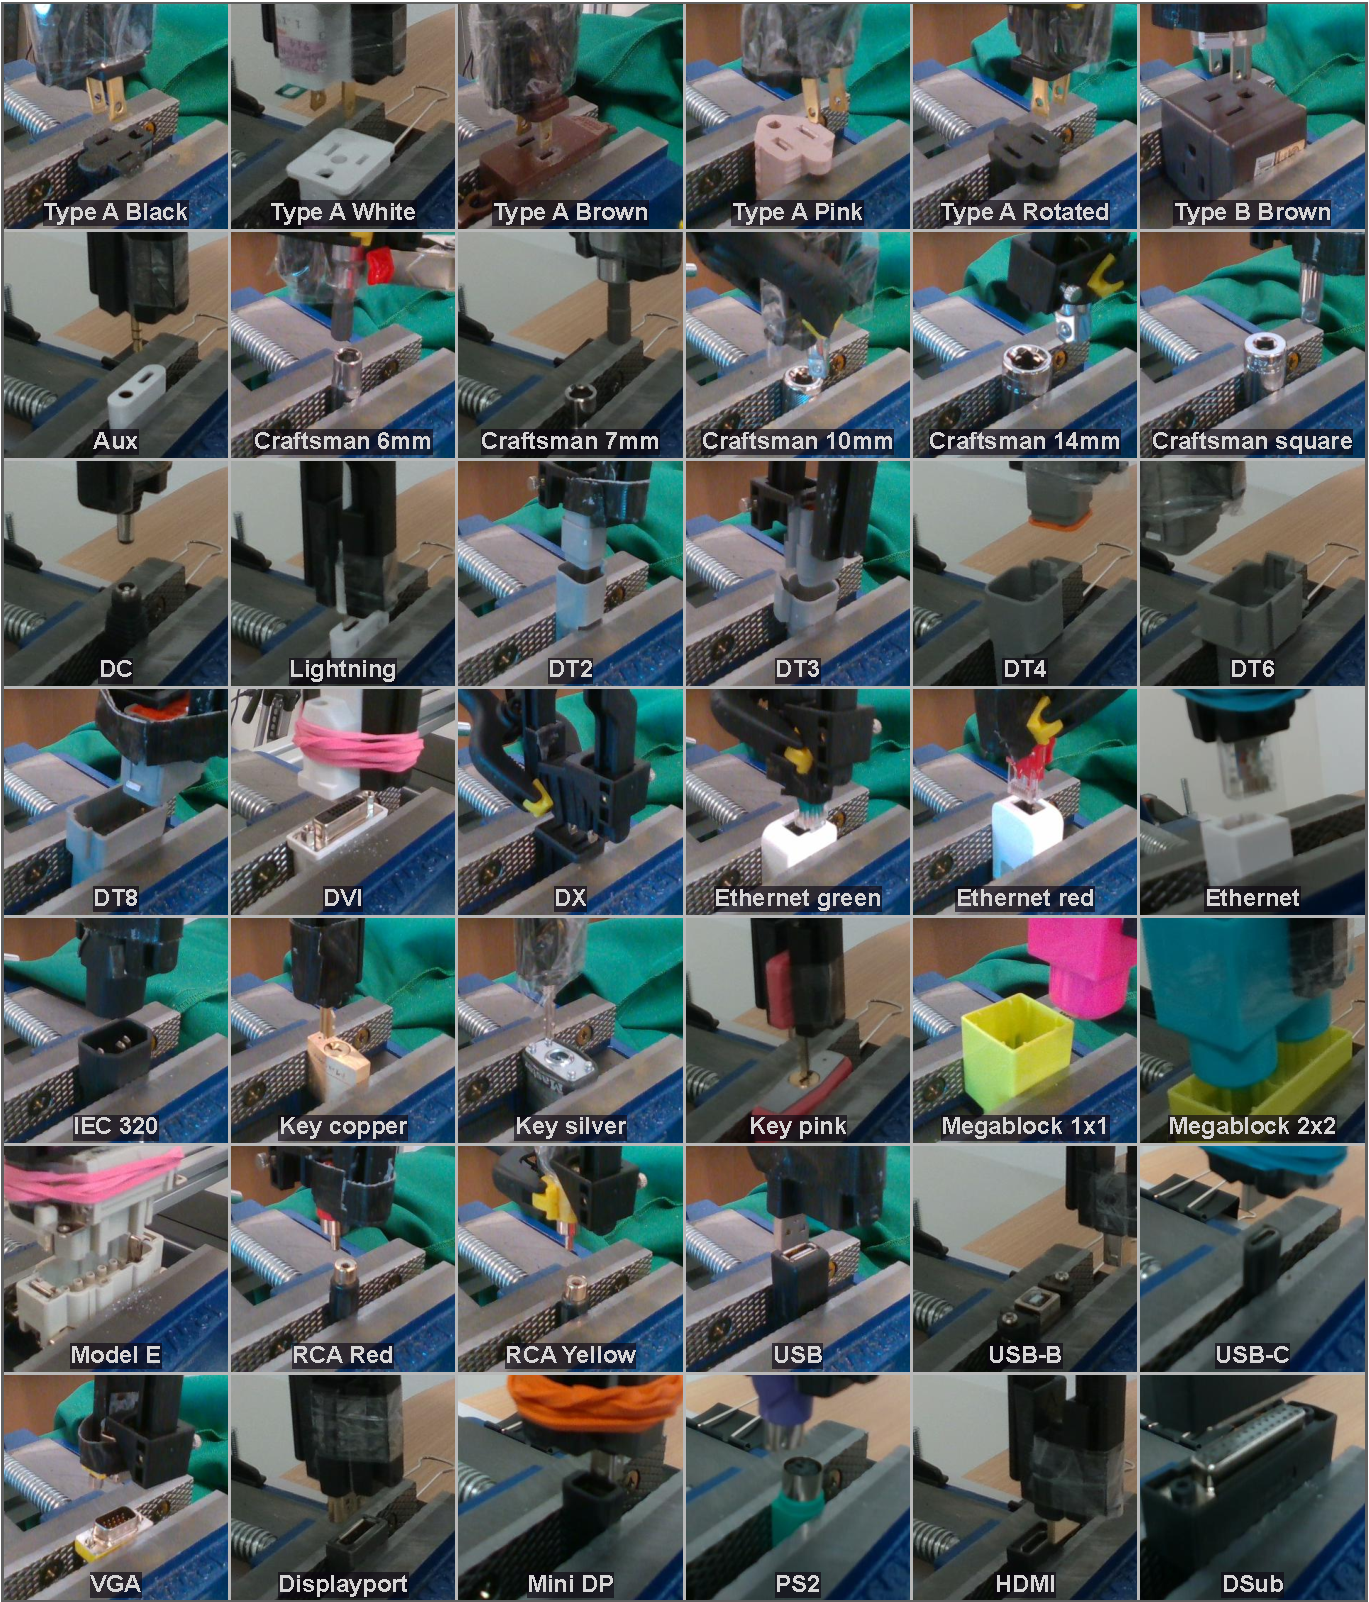
\includegraphics[width=0.99\textwidth]{imgs/connectors.pdf}
    \end{subfigure}

    \caption{Frames from our dataset of \numconnectors{} connectors.}
    \label{fig:connectortable}
    \vspace{-0.5cm}
% \end{wrapfigure}
\end{figure}

Our robot setup for connector insertion is pictured in Fig~\ref{fig:connectortable}. We use two 7 DoF Sawyer robots from Rethink Robotics for collecting data and running experiments. The robot is commanded with an end-effector controller, where the action $a$ corresponds to relative end-effector movement in Cartesian coordinates. The resulting desired joint angles are computed via inverse kinematics, and then executed with a joint-space velocity controller with force limits for safety and to prevent dislodging connectors from a grasped position.

We initially collect a dataset of insertions of \numconnectors{} connectors. For each connector, it is grasped by the robot and the socket is mounted to a clamp. Before data collection, the robot is manually placed in a successful grasp position and a calibration procedure captures the initial pose for detecting ground truth success. During data collection, the robot follows a manual insertion strategy of moving downwards if within 1mm of the center-line of the socket, and moving towards the center-line of the connector otherwise. Noisy actions are executed with probability $0.2$ to visit a diverse set of states and induce recovery behavior in the prior data.

We want to utilize this data to allow the robot to generalize to a held-out connector not seen during training.


\section{Experiments}


\renewcommand{\arraystretch}{1.4}
\setlength{\arrayrulewidth}{0.1mm}
\setlength{\tabcolsep}{3pt}

\begin{table}[]
% \small
\begin{tabular}{l|r|r|r|r|r|r}
Connector & \multicolumn{1}{l}{Localize} & \multicolumn{1}{l}{\begin{tabular}[c]{@{}l@{}}Straight\\ Down\end{tabular}} & \multicolumn{1}{l}{\begin{tabular}[c]{@{}l@{}}Random\\ Search\end{tabular}} & \multicolumn{1}{l}{\begin{tabular}[c]{@{}l@{}}Spiral\\ Search\end{tabular}} & \multicolumn{1}{l}{\begin{tabular}[c]{@{}l@{}}Ours\\ (offline)\end{tabular}} & \multicolumn{1}{l}{\begin{tabular}[c]{@{}l@{}}Ours\\ (online)\end{tabular}} \\ \hline \hline
DT12-1    & 3/20                         & 1/20                                                                        & 7/20                                                                        & 4/20                                                                        & 7/20                                                                         & 19/20                                                                 \\
Mega 1x1  & 3/20                         & 1/20                                                                        & 1/20                                                                        & 15/20                                                                       & 5/20                                                      & 16/20                                                  \\
NEMA 15   & 0/20                         & 1/20                                                                        & 0/20                                                                        & 3/20                                                                        & 11/20                                                                        & 15/20                                                                 \\
Europlug  & 6/20                         & 4/20                                                                        & 6/20                                                                        & 4/20                                                                        & 10/20                                                                        & 15/20                                                                
\end{tabular}
\caption{Insertion scenario I: the initial position of the gripper is located $\pm$10mm from the socket centered around the socket.}
\label{table:easy}
\end{table}



\renewcommand{\arraystretch}{1.4}
\setlength{\arrayrulewidth}{0.1mm}
\setlength{\tabcolsep}{3pt}

\begin{table}[]
% \footnotesize
\begin{tabular}{l|r|r|r|r|r|r}
Connector     & \multicolumn{1}{l}{Localize} & \multicolumn{1}{l}{\begin{tabular}[c]{@{}l@{}}Straight\\ Down\end{tabular}} & \multicolumn{1}{l}{\begin{tabular}[c]{@{}l@{}}Random\\ Search\end{tabular}} & \multicolumn{1}{l}{\begin{tabular}[c]{@{}l@{}}Spiral\\ Search\end{tabular}} & \multicolumn{1}{l}{\begin{tabular}[c]{@{}l@{}}Ours\\ (offline)\end{tabular}} & \multicolumn{1}{l}{\begin{tabular}[c]{@{}l@{}}Ours\\ (online)\end{tabular}} \\ \hline \hline
DT12-1        & 0/20                         & 0/20                                                                        & 0/20                                                                        & 0/20                                                                        & 0/20                                                                         & 18/20                                                                 \\
Mega 1x1 & 0/20                         & 1/20                                                                        & 0/20                                                                        & 17/20                                                                       & 0/20                                                                         & 20/20                                                                 \\
NEMA 15     & 0/20                         & 0/20                                                                        & 0/20                                                                        & 0/20                                                                        & 6/20                                                                         & 17/20                                                                 \\
Europlug      & 0/20                         & 0/20                                                                        & 0/20                                                                        & 0/20                                                                        & 2/20                                                                         & 15/20                                                                
\end{tabular}
\caption{Insertion scenario II: the initial position of the gripper is sampled from a box 10-20mm from the socket. This scenario is more difficult as moving straight down almost never solves the task. The baselines in this series of experiments use localization model initially, then follow the baseline strategy.}
\label{table:hard}
\end{table}

\renewcommand{\arraystretch}{1.4}
\setlength{\arrayrulewidth}{0.1mm}
\setlength{\tabcolsep}{3pt}


\renewcommand{\arraystretch}{1.4}
\setlength{\arrayrulewidth}{0.1mm}
\setlength{\tabcolsep}{3pt}

\begin{table}[]
\centering
\begin{tabular}{l|ll|rr}
         & Reward & Policy & \multicolumn{1}{l}{Offline} & \multicolumn{1}{l}{Online} \\ \hline \hline
DT12-1   & DAIB   & DAIB   & 0/20                           & 18/20                         \\
         & DAIB   & -      & 0/20                           & 4/20                          \\
         & -      & -      & 0/20                           & 0/20                          \\  \hline
Mega 1x1 & DAIB   & DAIB   & 0/20                           & 20/20                         \\
         & DAIB   & -      & 3/20                           & 20/20                         \\
         & -      & -      & 3/20                           & 0/20                          \\  \hline
NEMA 15  & DAIB   & DAIB   & 6/20                           & 17/20                         \\
         & DAIB   & -      & 0/20                           & 2/20                          \\
         & -      & -      & 0/20                           & 0/20                          \\  \hline
Europlug & DAIB   & DAIB   & 2/20                           & 15/20                         \\
         & DAIB   & -      & 1/20                           & 12/20                         \\
         & -      & -      & 0/20                           & 15/20                        
\end{tabular}
\caption{Ablation of using the domain adversarial information bottleneck (DAIB) for the reward and for the policy across all four test connectors. The only consistent setting where finetuning occurs across all four connectors is using the DAIB for both reward and policy. Removing the bottleneck for the policy significantly reduces finetuning performance on two tasks, but still finetunes on the other two. Removing the bottleneck for the reward prevents finetuning except for the Europlug connector. }
\end{table}


We design our experiments to answer the following questions.
\begin{itemize}
    \item Does the domain adversarial information bottleneck improve accuracy for reward classification?
    \item Can offline reinforcement learning followed by online fine-tuning be a solution for industrial insertion of novel connectors, and does it outperform a supervised localization model combined with a manually scripted control strategy?
    % \item Does vision-based RL outperform state-based methods in the presence of noise?
    % \item Is offline reinforcement required (as opposed to behavior cloning)?
    \item What is the model paying attention to?
    % \item Can the learned features transfer to a new robot?
\end{itemize}

\subsection{Reward Classification}

To learn a generalizable reward function and to evaluate the proposed domain generalization method, we first need to learn a reward classifier from the offline data. 
The accuracy of this reward classifier has a significant impact on whether online finetuning with the learned reward will successfully solve a task; if the reward is inaccurate, the policy can adversarially learn to go to regions of incorrect high reward.
We train the reward classifier on a subset of the data consisting of 25 connectors and evaluated on a set of five held-out connectors.
During training and evaluation, the data is rebalanced to be $50\%$ positive and $50\%$ negative samples per connector.
In Table~\ref{tab:reward}, we report the mean accuracy of each method averaged across the five held-out connectors.

We compare the following methods.
Our method, \textbf{DAIB} uses a domain adversarial objective in combination with a variational information bottleneck as detailed in section~\ref{sec:reward}. \textbf{DANN} enforces domain invariance using a domain adversarial neural network~\cite{ganin2016domainadversarial}. \textbf{DAIB, $\lambda=0$} adds an additional network path from the input image to the reward classifier as in DAIB, but without enforcing an information bottleneck. \textbf{VIB} enforces a variational information bottleneck only without domain invariance~\cite{alemi2017vib}. \textbf{ERM} has no auxiliary representation learning objectives.

\begin{wraptable}[13]{r}{3.5cm}
\begin{tabular}{l|l}
Method   & Acc. \\ \hline
DAIB (Ours) & \textbf{88\%}     \\
DANN          & 71\%     \\
DAIB, $\lambda=0$    & 77\%     \\
VIB         & 79\%     \\
ERM             & 76\%    
\end{tabular}
\caption{Comparison of test accuracy on reward classification.}
\label{tab:reward}
\end{wraptable}
The results are presented in Table~\ref{tab:reward}. We see that our method, DAIB, is able to achieve an $88\%$ accuracy, significantly higher than other methods. DANN, which enforces domain invariance, is the worst performing. This poor performance shows that the domain invariance assumption is too strong for the task of reward classification; connector insertion does require domain-specific information. The DANN + no VIB
%%should we call this DAIB, lambda=0
method achieves similar accuracy as ERM, since the network can just make the domain invariant features degenerate and bypass the domain adversarial objective.
The VIB alone slightly improves performance over ERM because of a regularizing effect. But all methods achieve significantly worse accuracy than DAIB. Next, armed with an accurate reward model, we investigate finetuning connectors using the learned reward model.

% \begin{table}[]
% \begin{tabular}{l|l}
% Representation   & Accuracy \\ \hline
% DAIB (Ours) & \textbf{88\%}     \\
% DANN          & 71\%     \\
% DANN + no VIB      & 77\%     \\
% VIB         & 79\%     \\
% ERM             & 76\%    
% \end{tabular}
% \caption{Reward classifier results}
% \label{tab:reward}
% \end{table}

\begin{figure*}[t]
    \centering
    \begin{subfigure}[b]{0.99\linewidth}
        \center
        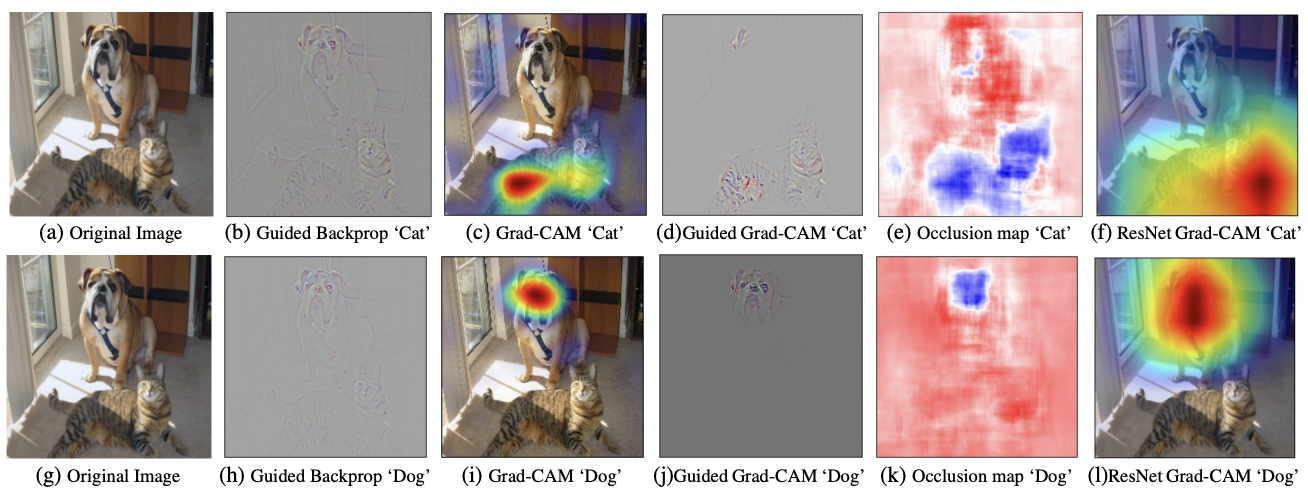
\includegraphics[width=0.99\textwidth]{imgs/gradcam_placeholder.png}
    \end{subfigure}

    \caption{[PLACEHOLDER FOR NETWORK INSPECTION EXPERIMENTS] 1. policy is playing attention to corresponding edges of connectors, and localization doesn't pay attention to something sensible and/or 2. DAIB bottleneck makes this happen more often than non-DAIB, for policy and/or reward}

    \label{fig:novel_obj}
    \vspace{-0.5cm}
% \end{wrapfigure}
\end{figure*}

\subsection{Self-Supervised Fine-tuning}

For insertion of a novel connector, we first run offline training of RL on a set of connectors excluding that connector or close variants (eg. same connector on a different robot), to obtain a policy, Q function, and value function.
Then, we run online finetuning of RL on the novel connector.
We evaluate four connector insertion tasks: a Deutsch DT 12-way connector, a Megablock, a NEMA 15-5 connector, and a Europlug connector.
We also evaluate in two settings: a relatively easier scenario where the initial location of the connector is centered around the socket with $\pm10mm$ noise, and a harder scenario where the initial location of the connector is offset from the socket by $10-20mm$.

In the easier $\pm10mm$ setting, we compare against the four following baselines. \textbf{Localize}: regress on to the state positions in the same offline data at each step and execute an expert policy towards that goal location which moves horizontally until within $1mm$ of the goal, then move straight down. \textbf{Straight down}: move straight down from the starting position. \textbf{Random search}: from the initial starting position, move straight down and then move to 5 randomly sampled positions while pressing down. \textbf{Spiral search}: from the initial starting position, move straight down and then move in a spiral while pressing down. Each method including ours is executed for 20 time steps per trajectory for evaluation.

The results are reported in Table~\ref{table:easy}. We see that the performance of most methods are inconsistent, but DAIB online successfully solves the task to $>75\%$ success for all four connectors.

In the harder $10-20mm$ setting, we compare against similar baselines but straight down, random search, and spiral search from the initial position always fail because the initial position is too far away from the socket. Instead, for these three methods, we first execute the localization model and move to that goal position, then run the corresponding strategy.

The results for the harder insertion scenario is reported in Table~\ref{table:hard}. In this case, the performance of most methods, including DAIB offline, on most connectors, is poor. However, DAIB online is able to solve these tasks after 200 trials of finetuning. Importantly, even when the initial performance is 0/20 as in the DT 12-way connector, DAIB can improve because of well-shaped value functions guiding the policy towards the correct solution. In practice, we see that even when the initial policy is poor and does not get close to the socket, the finetuned policy quickly makes contact with the socket within a few trials. Then more trials are required to actually observe successes through stochastic exploration to perfect the policy.

% \subsection{Effect of Vision}


% Better than state-based training? - with this amount of variation, it definitely is

% \subsection{Reinforcement Learning vs IQL}

% Is offline RL better than BC?

% Could show some value function

% Better than basic representation learning methods? Eg. contrastive / ImageNet pretraining / reconstructive

\subsection{Inspecting the Networks}

Inspecting the learned features - does it focus on edges to line up in a scene, etc.?

% \subsection{Generalizable Reward Functions}

% Can the learned features transfer to a new robot? (evaluate reward prediction accuracy)

% \begin{table}
% \begin{tabular}{l|c|c|c|c|c}
% & \multicolumn{3}{c|}{Plug} & \multicolumn{2}{c}{Gear} \\
% Policy &  0 & $\pm2$mm & $\pm3$mm & 0 & $\pm2$mm  \\ \hline
% \multirow{2}{*}{Straight Down} & $\textbf{3.3}$ & $-$ & $-$ & $\textbf{5.3}$ & $-$ \\
% & $\pm0.6$ & & & $\pm1.4$ & \\
% \hline
% \multirow{2}{*}{Random Search} & 5.6 & $\textbf{7.0}$ & $\textbf{9.7}$ & 20.3 & $23.3$ \\
% & $\pm2.0$ & $\pm2.3$ & $\pm4.6$ & $\pm7.3$ & $\pm9.3$ \\
% \hline
% \multirow{2}{*}{Spiral-Search} &  $6.0$ &  $13.6$ & $26.6$ & $8.0$ & $17.3$ \\
% & $\pm4.7$ & $\pm6.6$ & $\pm4.8$ & $\pm2.6$ & $\pm5.2$ \\
% \hline
% \multirow{2}{*}{RL from Scratch} &  $11.7$ & $-$ & $-$ & $\textbf{5.8}$ & $-$\\
% & $\pm 4.2$ & & & $\pm 0.7$ & \\
% \hline
% \multirow{2}{*}{PEARL Sim2Real} & $5.3$ & $\textbf{6.8}$ & $\textbf{8.2}$& $\textbf{5.7}$ & $\textbf{8.0}$ \\
% & $\pm2.7$ & $\pm4.7$ & $\pm4.5$ & $\pm2.6$ & $\pm5.5$ \\
% \end{tabular}
% \vspace{-0.4cm}
% \label{tab:success_rates}
% \end{table}

% \begin{figure}[t]
%     \centering
%     \begin{subfigure}[b]{0.99\linewidth}
%         \center
%         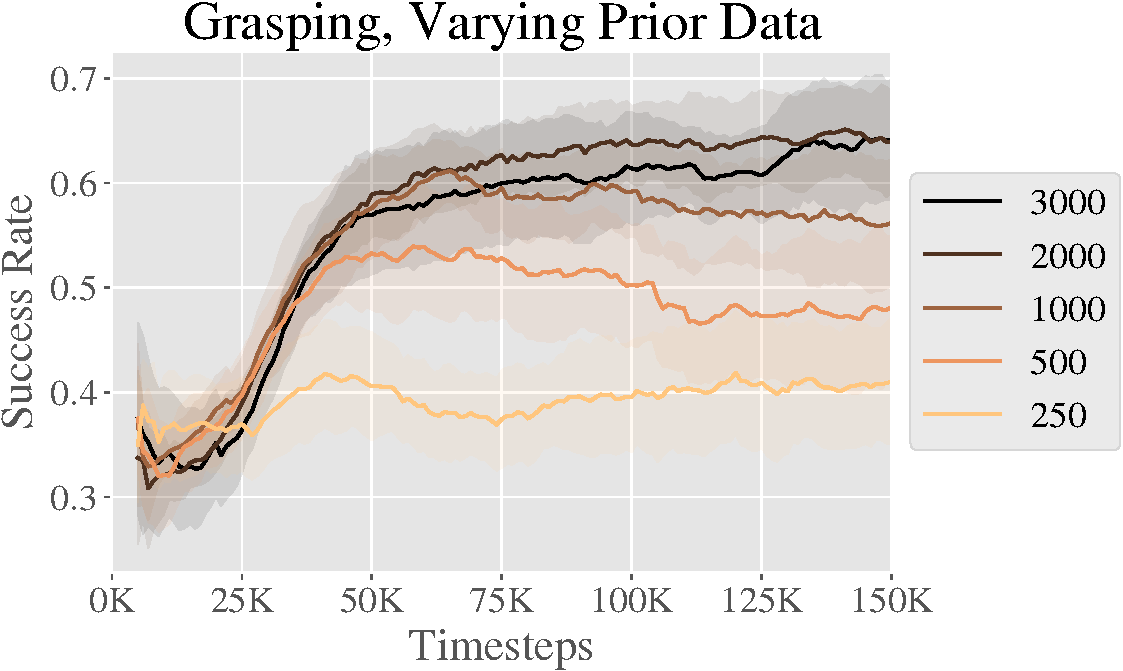
\includegraphics[width=0.6\textwidth]{imgs/vary_data-crop.pdf}
%     \end{subfigure}

%     \caption{[PLACEHOLDER FROM PREVIOUS WORK - VAL] Learning curves for simulated grasping of novel objects with VAL, using data from an increasing number of training objects for offline RL. We collect 50 trajectories per training object, and each line is labeled with the total number of training trajectories. \textit{We want to show something similar on real-world connectors.} }

%     \label{fig:novel_obj}
%     \vspace{-0.5cm}
% % \end{wrapfigure}
% \end{figure}

\section{Discussion}



\IEEEtriggeratref{28} % \newpage after bib reference 28

{ \small
% \bibliographystyle{corlabbrvnat}
\bibliographystyle{IEEEtran}
\bibliography{example}
}

\end{document}
